\chapter{ROS 2 Middleware Implementation for WebAssembly}

    The design of a custom middleware implementation, \textsf{rms\_wasm}, that can be cross-compiled to WebAssembly modules is divided into three distinct packages as observed in Figure~\ref{fig:rmwwasm}. For this project, these packages were developed in the order shown, starting with \textsf{rmw\_wasm\_cpp}.

    \begin{figure}[htbp]
        \centering
        \vspace{1em}
        \begin{tikzpicture}
            \node (pkg) [
                rectangle,
                rounded corners,
                draw = textColor,
                fill = igmrLightBlue!10!bgColor,
                text height = 7cm,
                align = justify,
                minimum width = 14cm,
                text width = 13.5cm,
            ] {\textsf{rmw\_wasm}};

            \node (rwc) [
                packBox,
                yshift = 2.5cm,
                fill = igmrLightBlue!30!bgColor,
                ] {\textsf{rmw\_wasm\_cpp}};

            \node (wcpp) [
                packBox,
                yshift = 0.5cm,
                fill = igmrLightBlue!30!bgColor,
                ] {\textsf{wasm\_cpp}};

            \node (wjs) [
                packBox,
                yshift = -2.5cm,
                fill = igmrLightBlue!30!bgColor,
                ] {\textsf{wasm\_js}};
            
            \node (ems) [
                rectangle,
                yshift = -1cm,
                xshift = 1.5cm,
                ] {\textsf{emscripten::val}};

            \draw[thick] (rwc) -- (wcpp);
            \draw[thick] (wcpp) -- (wjs);

        \end{tikzpicture}
        \vspace{1em}
        \caption{Architecture of custom middleware implementation to target WebAssembly.}
        \label{fig:rmwwasm}
    \end{figure}

    \section{rmw\_wasm\_cpp}

        The first package, \textsf{rmw\_wasm\_cpp}, works as the ``adapter'' between \ac{ROS} 2 and the designed middleware. This package implements all of the functions required for \textsf{rmw} as described in Section~\ref{ssec:minimal}. The source code for this package is entirely written in C++ and can be found: TODO: 

        TODO: add diagram

        TODO: mention yaml conversion, add diagram?

    \section{wasm\_cpp}

        The role of \textsf{wasm\_cpp} is to implement the middleware and to function as a bridge to JavaScript modules. This package, along with \textsf{wasm\_js} constitute the middleware implementation without the adapter, and thus, they can function independently of \textsf{rmw\_wasm\_cpp}. 

        The \ac{ROS} elements in this package build on top of each other, where the smallest unit is a \textsf{Participant}. Any \ac{ROS} subscriber, publisher, service server, service client, action server, or action client is simply a \textsf{Participant} with a specific role. Each \textsf{Participant} must have a valid name which follows the \ac{ROS} guidelines (TODO: add ref for valid names). For publishers and subscribers, this name is their respective topic name. And for servers and clients, the name corresponds to the service or action name.  Upon initialization, each \textsf{Participant} also receives a unique ID or \textsf{gid} which is used to keep track of individual participants. 

        Subscribers and publishers are the simplest type of participants. And each of them only has one function; a publisher needs to be able to \textit{publish} a message, and a subscriber must be able to \textit{retrieve} the message from a specific topic. The messages which the publisher handles are yaml strings. These messages are then passed to \textsf{wasm\_js} by using \textsf{emscripten::val} which transliterates JavaScript code into C++ (TODO: add ref). Figure~\ref{fig:publish} shows how these functions are implemented to create a \textit{bridge} between the two packages.

        \begin{figure}[htbp]
            \centering
            \begin{lstlisting}[language=C++]
// wasm_cpp/src/publisher.cpp
#include <emscripten/emscripten.h>
#include <emscripten/val.h>
...
emscripten::val js_publish = emscripten::val::module_property("publishMessage");
bool is_published = js_publish(yaml_message, topic_name).as<bool>();
\end{lstlisting}

            % To match syntax hightlight
            \begin{lstlisting}[language=C++] 
// wasm_js/src/pre.js
Module["publishMessage"] = function publishMessage(message, topic_name)
{
    // Send message to main
    if (message.startsWith("data:")) {
    self.postMessage({
        command: "publish",
        topic:    topic_name,
        message: message
    });
    }

    return true;
}
\end{lstlisting}
            \caption{Publisher sending a message to JavaScript for publishing.}
            \label{fig:publish}
        \end{figure}

    Conversely, the subscriber \textit{waits} for a response from \textsf{wasm\_js} which will indicate that a new message has been published to the topic in question. The response message type is coerced into a yaml string to send back to \textsf{rmw\_wasm\_cpp}. This process is illustrated in Figure~\ref{fig:retrieve}.

    \begin{figure}[htbp]
        \centering
        \begin{lstlisting}[language=C++]
// wasm_cpp/src/subscriber.cpp
emscripten::val js_retrieve = emscripten::val::module_property("retrieveMessage");
emscripten::val js_response = js_retrieve(topic_name).await();
std::string yaml_message = js_response.as<std::string>();
\end{lstlisting}    
        \caption{Subscriber retrieving a message from JavaScript.}
        \label{fig:retrieve}
    \end{figure}

    \begin{figure}[htbp]
        \centering
        \begin{tikzpicture}%[show background grid]
            \begin{abstractclass}[text width=5cm]{Participant}{0,0}
                \attribute{- name : String}
                \attribute{- role : String}
                \attribute{- gid  : String}

                \operation{- is\_valid\_name()}
                \operation{- is\_valid\_role()}
                \operation{- registration()}
                \operation{- deregistration()}
            \end{abstractclass}

            \begin{class}[text width=5cm]{Publisher}{-5,-6}
                \inherit{Participant}
                \attribute{- name = topic\_name}
                \attribute{- role = publisher}
                \operation{+ publish(message : String)}
            \end{class}

            \begin{class}[text width=5cm]{Subscriber}{5,-6}
                \inherit{Participant}
                \attribute{- name = topic\_name}
                \attribute{- role = subscriber}
                \operation{+ get\_message() : String}
            \end{class}

            \begin{class}[text width=6.5cm]{ServiceServer}{-4,-11}
                \inherit{Participant}
                \attribute{- name = service\_name}
                \attribute{- role = service\_server}
                \operation{+ take\_request() : String}
                \operation{+ send\_response(response : String)}
            \end{class}

            \composition{ServiceServer}{}{}{Publisher}
            \composition{ServiceServer}{}{}{Subscriber}

            \begin{class}[text width=6.5cm]{ServiceClient}{4,-11}
                \inherit{Participant}
                \attribute{- name = service\_name}
                \attribute{- role = service\_client}
                \operation{+ send\_request(request : String)}
                \operation{+ take\_response() : String}
                \operation{+ is\_service\_available() : Bool}
            \end{class}

            \composition{ServiceClient}{}{}{Publisher}
            \composition{ServiceClient}{}{}{Subscriber}

        \end{tikzpicture}
        \caption{A class diagram}
    \end{figure}
    
    \section{wasm\_js}


    \subsection{Web Workers}

        
        \begin{figure}[htbp]
            \centering
            \begin{tikzpicture}
                \node (thread) [
                    rectangle,
                    rounded corners,
                    draw = textColor,
                    text depth = 4cm,
                    minimum width = 4cm,
                    fill = igmrLightBlue!30!bgColor,
                ] {Main Thread};

                \node (w1) [
                    webBox,
                    xshift = -5cm,
                    yshift = 1cm,
                ] {ROS Node 1 \\ \footnotesize{web worker}};

                \node (w2) [
                    webBox,
                    xshift = -5cm,
                    yshift = -2cm,
                ] {ROS Node 2 \\ \footnotesize{web worker}};

                \node (w3) [
                    webBox,
                    xshift = 5cm,
                    yshift = 1cm,
                ] {ROS Node 3 \\ \footnotesize{web worker}};

                \node (w4) [
                    webBox,
                    xshift = 5cm,
                    yshift = -2cm,
                ] {ROS Node 4 \\ \footnotesize{web worker}};

            \end{tikzpicture}
            \caption{TODO: Web Worker communications}
            \label{fig:webworker}
        \end{figure}

        

    \subsection{Message Stacks}

        \begin{figure}[htbp]
            \centering
            \begin{subfigure}[t]{0.32\textwidth}
                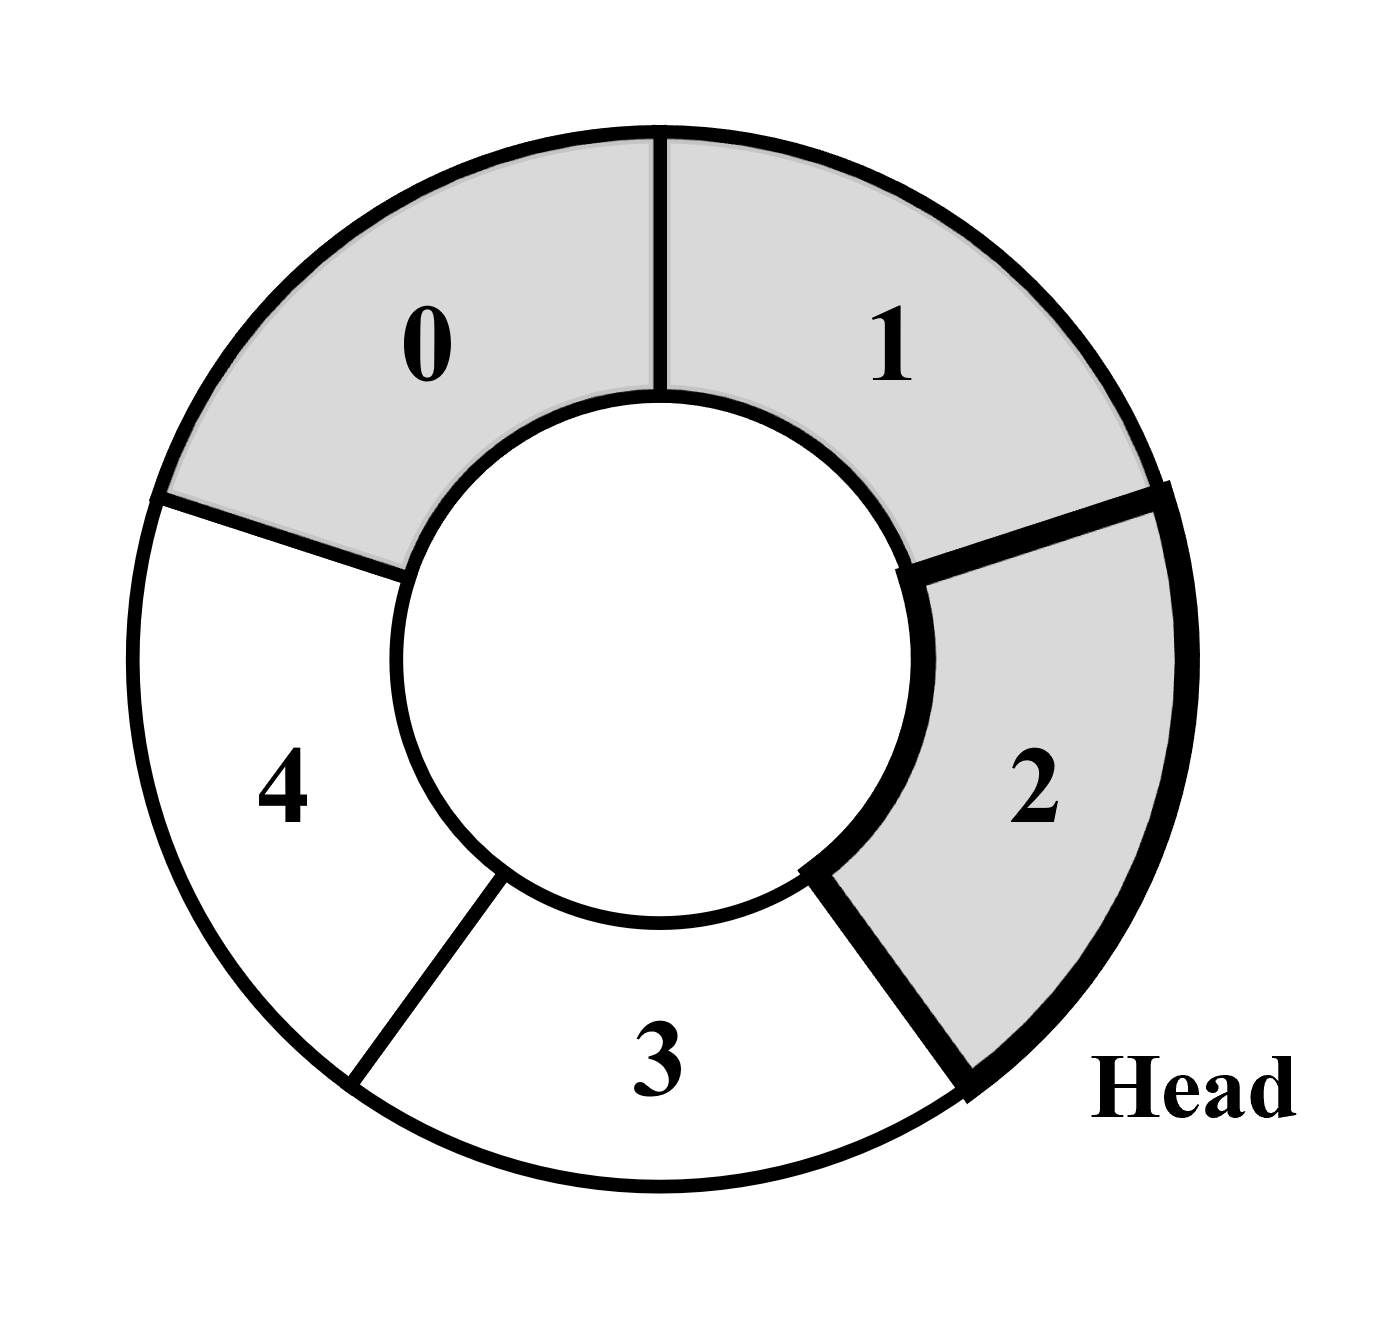
\includegraphics[height=0.9\textwidth]{07_stack0.png}
                \caption{Filling stack}
            \end{subfigure}
            \begin{subfigure}[t]{0.32\textwidth}
                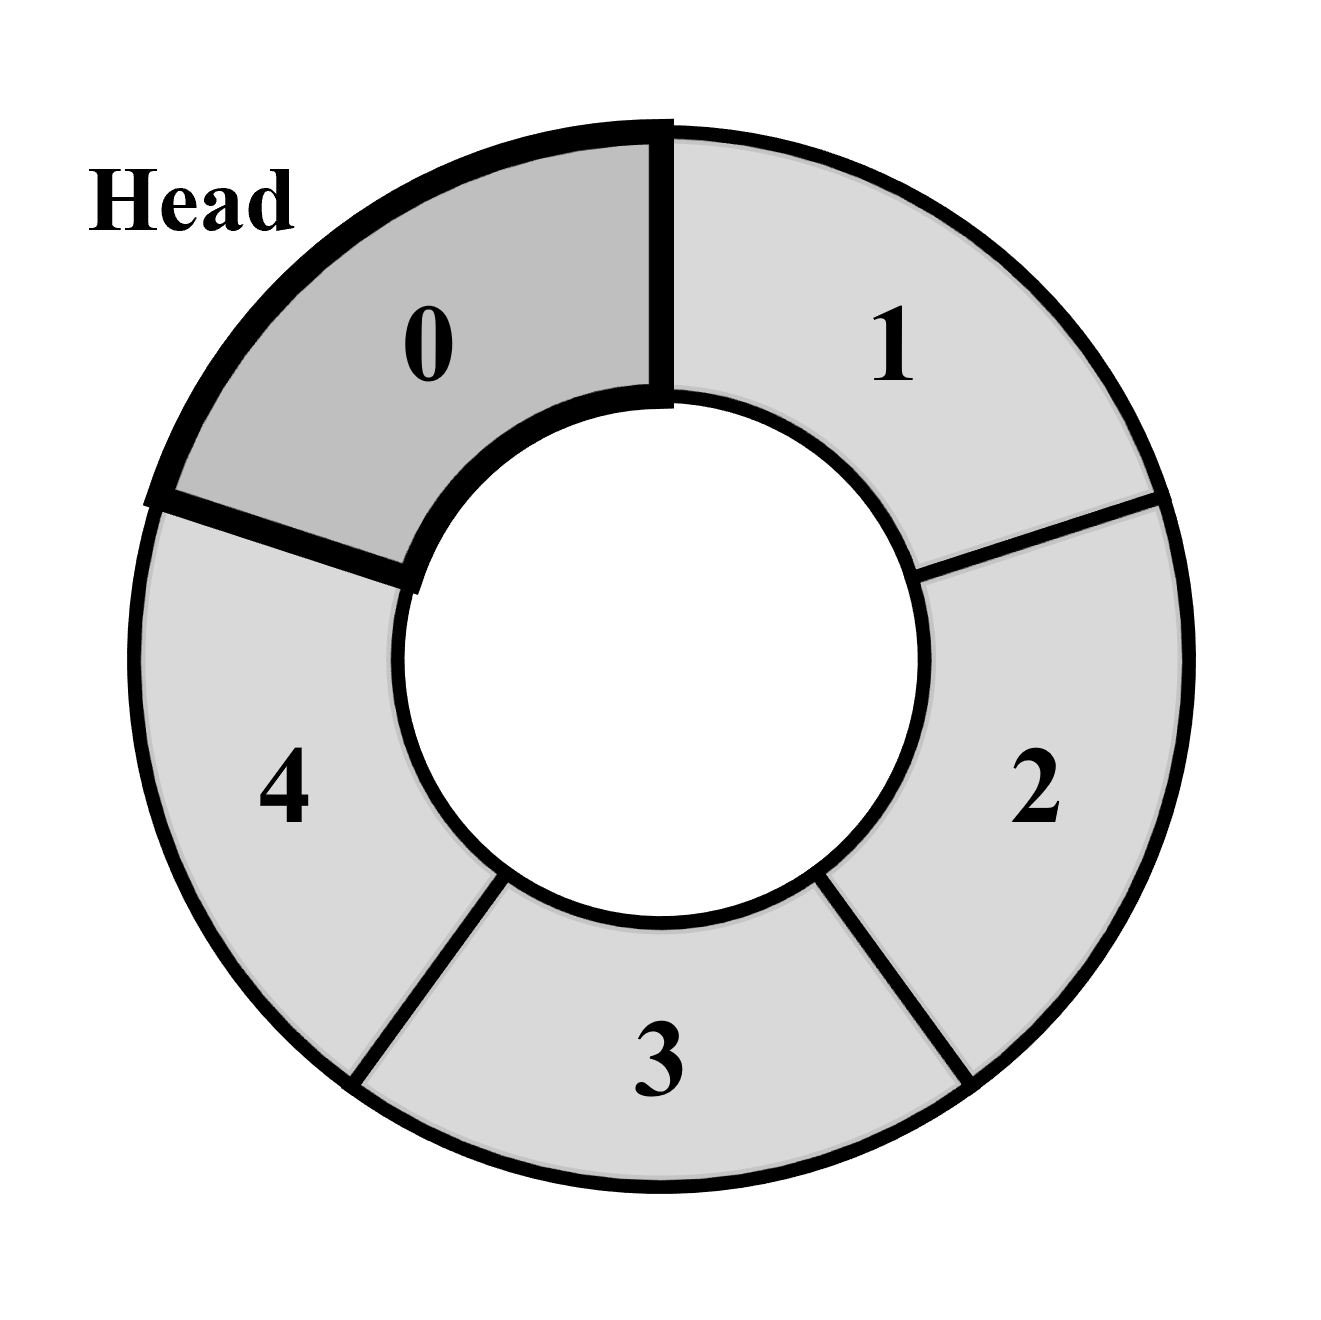
\includegraphics[height=0.9\textwidth]{07_stack1.png}
                \caption{Overwriting stack}
            \end{subfigure}
            \begin{subfigure}[t]{0.32\textwidth}
                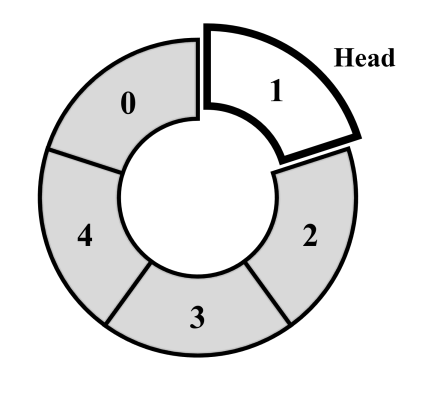
\includegraphics[height=0.9\textwidth]{07_stack2.png}
                \caption{Reading stack}
            \end{subfigure}
            \caption{Modified Circular Stack, \ac{LIFO}}
            \label{fig:circleStack}
        \end{figure}

    - Web workers, what are they? why are they needed?
    - Communication channels
    - Registry of topics/subs/pubs
    - Message handling

